%% Follow comments to support use.

%%%%%%%%%%%%%%%%%%%%%%%%%%%%%%%%%%%%%%%%%%%%%%%%%%%%%%%%%
%% STEP 1: Choose options for MSc / BSc / seminar layout and your bibliographic style
%%%%%%%%%%%%%%%%%%%%%%%%%%%%%%%%%%%%%%%%%%%%%%%%%%%%%%%%%

%%  Language:
%%      finnish, swedish, or english
%%  Pagination (use twoside by default)
%%      oneside or twoside,
%%  Study programme / kind of report
%%      csm  = Master's thesis in Computer Science Master's Programme;
%%      tkt = Bachelor's thesis in Computer Science Bachelor's Programme;
%%      seminar = seminar report
%%  For Master's thesis choose your line or track:
%%      (30 cr thesis, 2020 onwards, Master's Programme in Computer Science = csm)
%%      software-track-2020 = Software study track
%%      algorithms-track-2020 = Algorithms study track
%%      networking-track-2020 = Networking study track

\documentclass[finnish,twoside,censored,tkt]{HYthesisML}
%\documentclass[english,twoside,censored,tkt]{HYthesisML}

% If wanted, open new chapters only at right page.
% By default, "openany".
%\PassOptionsToClass{openright,twoside,a4paper}{report}
\PassOptionsToClass{openany,twoside,a4paper}{report}

\usepackage{csquotes}
%%%%%%%%%%%%%%%%%%%%%%%%%%%%%%%%%%%%%%%%%%%%%%%%%%%%%%%%%
%% REFERENCES
%% Some notes on bibliography usage and options:
%% natbib -> you can use, e.g., \citep{} or \parencite{} for (Einstein, 1905); with APA \cite -> Einstein, 1905 without ()
%% maxcitenames=2 -> only 2 author names in text citations, if more -> et al. is used
%% maxbibnames=99 as no great need to suppress the biliography list in a thesis
%% for more information see biblatex package documentation, e.g., from https://ctan.org/pkg/biblatex

%% Reference style: select one
%% for APA = Harvard style = authoryear -> (Einstein, 1905) use:
\usepackage[style=authoryear,bibstyle=authoryear,backend=biber,natbib=true,maxnames=99,maxcitenames=2,uniquelist=minyear,giveninits=true,uniquename=mininit,dashed=false]{biblatex}
%% for numeric = Vancouver style -> [1] use:
%\usepackage[style=numeric,bibstyle=numeric,backend=biber,natbib=true,maxbibnames=99,giveninits=true,uniquename=init]{biblatex}


\addbibresource{bibliography.bib}
% in case you want the final delimiter between authors & -> (Einstein & Zweistein, 1905)
% \renewcommand{\finalnamedelim}{ \& }
% List the authors in the Bibilipgraphy as Lastname F, Familyname G,
\DeclareNameAlias{sortname}{family-given}
% remove the punctuation between author names in Bibliography
%\renewcommand{\revsdnamepunct}{ }


%% Block of definitions for fonts and packages for picture management.
%% In some systems, the figure packages may not be happy together.
%% Choose the ones you need.

%\usepackage[utf8]{inputenc} % For UTF8 support, in some systems. Use UTF8 when saving your file.

\usepackage{lmodern}         % Font package, again in some systems.
\usepackage{textcomp}        % Package for special symbols
\usepackage[pdftex]{color, graphicx} % For pdf output and jpg/png graphics
\usepackage{epsfig}
\usepackage{subfigure}
\usepackage[pdftex, plainpages=false]{hyperref} % For hyperlinks and pdf metadata
\usepackage{fancyhdr}        % For nicer page headers
\usepackage{tikz}            % For making vector graphics (hard to learn but powerful)
%\usepackage{wrapfig}        % For nice text-wrapping figures (use at own discretion)
\usepackage{amsmath, amssymb} % For better math

% Custom packages added
\usepackage{dsfont}
\usepackage{xcolor}

\singlespacing               %line spacing options; normally use single

\fussy
%\sloppy                      % sloppy and fussy commands can be used to avoid overlong text lines
% if you want to see which lines are too long or have too little stuff, comment out the following lines
% \overfullrule=1mm
% to see more info in the detailed log about under/overfull boxes...
% \showboxbreadth=50
% \showboxdepth=50



%%%%%%%%%%%%%%%%%%%%%%%%%%%%%%%%%%%%%%%%%%%%%%%%%%%%%%%%%
%% STEP 2:
%%%%%%%%%%%%%%%%%%%%%%%%%%%%%%%%%%%%%%%%%%%%%%%%%%%%%%%%%
%% Set up personal information for the title page and the abstract form.
%% Replace parameters with your information.
\title{Oppijan kehittymisen tukeminen oppimisanalytiikalla Moodlessa}

\author{Tuomas Alanen}
\date{\today}

% Set supervisors, use the titles according to the thesis language
% in English Prof. or Dr., or in Finnish toht. or tri or FT, TkT, Ph.D. or in Swedish...
% Include both advisors and supervisors in the same entry to get them appear on the abstract page.
% For MSc theses, the terms have somehow changed to supervisors and examiners, denoting BSc level advisors and supervisors. An unfortunate mismatch for now.
% Advisors for BSc theses and supervisors for MSc theses are the first contacts, supervisors for BSc theses and examiners for MSc theses are less visible but are responsible on % grading the works.

\supervisors{Lea Kutvonen}

\keywords{learning analytics, Moodle}
\additionalinformation{\translate{\track}}

%% For seminar reports:
%%\additionalinformation{Name of the seminar}

%% Provide classification terms, to appear on the abstract page.
%% Replace the classification terms below with the ones that match your work.
%% ACM Digital library provides a taxonomy and a tool for classification
%% in computer science. Use 1-3 paths, and use right arrows between the
%% about three levels in the path; each path requires a new line.

\classification{\protect{\ \\
\ Information systems $\rightarrow$ Information systems applications $\rightarrow$ Decision support systems $\rightarrow$ Data analytics
}}

%% If you want to quote someone special. You can comment this line out and there will be nothing on the document.
%\quoting{Bachelor's degrees make pretty good placemats if you get them laminated.}{Jeph Jacques}


%% OPTIONAL STEP: Set up properties and metadata for the pdf file that pdfLaTeX makes.
%% Your name, work title, and keywords are recommended.
\hypersetup{
    unicode=true,           % to show non-Latin characters in Acrobat’s bookmarks
    pdftoolbar=true,        % show Acrobat’s toolbar?
    pdfmenubar=true,        % show Acrobat’s menu?
    pdffitwindow=false,     % window fit to page when opened
    pdfstartview={FitH},    % fits the width of the page to the window
    pdftitle={},            % title
    pdfauthor={},           % author
    pdfsubject={},          % subject of the document
    pdfcreator={},          % creator of the document
    pdfproducer={pdfLaTeX}, % producer of the document
    pdfkeywords={something} {something else}, % list of keywords for
    pdfnewwindow=true,      % links in new window
    colorlinks=true,        % false: boxed links; true: colored links
    linkcolor=black,        % color of internal links
    citecolor=black,        % color of links to bibliography
    filecolor=magenta,      % color of file links
    urlcolor=cyan           % color of external links
}

%%-----------------------------------------------------------------------------------

\begin{document}

% Generate title page.
\maketitle

%%%%%%%%%%%%%%%%%%%%%%%%%%%%%%%%%%%%%%%%%%%%%%%%%%%%%%%%%
%% STEP 3:
%%%%%%%%%%%%%%%%%%%%%%%%%%%%%%%%%%%%%%%%%%%%%%%%%%%%%%%%%
%% Write your abstract in the separate file, to be positioned here.
%% You can make several abstract pages (if you want it in different languages),
%% in which case you should also define the language of the abstract,
%% as below.

% !TEX root = ./HY-CS-main.tex
\begin{abstract}

Nykypäivänä opetuksen tukena oppilaitoksissa hyödynnetään useita erilaisia verkkopalveluita. Yhteistä jokaiselle näistä palveluista on, että ne tallentavat tietoa käyttäjän toiminnasta sekä käyttäjän suorituksien arvioinneista. Tämän tutkielman tavoitteena on perehtyä mahdollisuuksiin hyödyntää tätä tietoa oppijan oppimistuloksien sekä opetuksen parantamiseksi.

Tutkielmassa tarkastellaan oppimisen analysoimisen tarpeita ja miksi oppimisanalytiikkaa halutaan tehdä. Lisäksi tarkastellaan Moodlea datalähteenä oppimisanalytiikalle sekä tutustutaan tarkemmin kahteen erilaiseen oppimisanalytiikassa käytettyyn tietomalliin. Lopuksi tarkastellaan kuinka oppimisanalytiikan avulla voidaan tietolähteiden avulla muodostaa oppijaa sekä opetusta tukevia analyysejä.

\end{abstract}

\begin{otherlanguage}{english}
\begin{abstract}

\end{abstract}
\end{otherlanguage}


% Place ToC
%\newpage
\mytableofcontents

\mainmatter

%%%%%%%%%%%%%%%%%%%%%%%%%%%%%%%%%%%%%%%%%%%%%%%%%%%%%%%%%
%% STEP 4: Write the thesis.
%%%%%%%%%%%%%%%%%%%%%%%%%%%%%%%%%%%%%%%%%%%%%%%%%%%%%%%%%
%% Your actual text starts here. You shouldn't mess with the code above the line except
%% to change the parameters. Removing the abstract and ToC commands will mess up stuff.
%%
%% Command \include{file} includes the file of name file.tex.
%% A new page will be created at every \include command,
%% which makes it appropriate to use it for large entities such as book chapters. Cannot be nested.
%% It is useful for a big project, as changing one of the include targets
%% won't force the regeneration of the outputs of all the rest.
%% Alternatively, \input is a more lower level macro
%% which simply inputs the content of the given file like it was copy&pasted there manually.

%% Change your chapter titles within these files and add the actual text in them.

% !TEX root = ./HY-CS-main.tex
\chapter{Johdanto\label{johdanto}}

Nykypäivänä opetuksen tukena oppilaitoksissa hyödynnetään useita erilaisia verkkopalveluita. Tälläisiä verkkopalveluita on esimerkiksi Moodle, ItsLearning tai Thinglink. Yhteistä jokaiselle näistä palveluista on, että ne tallentavat tietoa käyttäjän toiminnasta sekä hänen tekemien suorituksien arvioinneista. Kuinka näiden järjestelmien keräämä tietoaineisto voidaan hyödyntää oppijan avuksi? Tämän tutkielman tavoitteena on perehtyä mahdollisuuksiin hyödyntää tätä tietoa oppijan oppimistuloksien parantamiseksi.

Tahtotilana on muodostaa käsitys siitä, kuinka oppijalle voidaan esittää hänen oma toimintansa oppimisen eteen selkeässä helposti ymmärrettävässä muodossa. Tämän tarkoituksena on tarjota mahdollisuus ymmärtää omaa toimintaa sekä antaa mahdollisuuksia kehittää omaa toimintaa sen seurauksena. Päästäksemme tähän halutaan löytää oppijan käyttäytymisestä erilaisia malleja, joiden avulla pystyttäisiin havaitsemaan esimerkiksi oppijan tarvitseman tuki tai löytämään esimerkiksi isommassa kuvassa tarve kohdistaa lisää opetusta osaamisvajeen paikkaamiseksi.

Tutkielman toisessa luvussa \emph{\nameref{luku2}} tarkastellaan oppimisen analysoimisen tarpeita ja miksi oppimisanalytiikkaa halutaan tehdä. Luvussa käsitellään oppimisanalytiikan rakennetta sekä kuinka oppimisanalytiikka toteutuu käytännössä. Muodostetaan käsitys kuinka oppimisanalytiikka muodostaa syklin, joka tuottaa koko ajan näkymän oppimiseen.

Kolmannessa luvussa \emph{\nameref{luku3}} tarkastellaan Moodlea datalähteenä oppimisanalytiikalle sekä tutustutaan tarkemmin kahteen erilaiseen oppimisanalytiikassa käytettyyn tietomalliin. Moodlen osalta nostetaan esille aktiviteettien merkitys datalähteenä analyysimalleille. Luvussa myös tarkastellaan Naiivin Bayesin mallin sekä regressioanalyysin toteuttamista.

Neljännessä luvussa \emph{\nameref{luku4}} tarkastellaan kuinka oppimisanalytiikan avulla voidaan datalähteiden avulla muodostaa oppijaa sekä opetusta tukevia analyysejä. Luvussa tuodaan esille kuinka oppija, opettaja sekä hallintohenkilöstö pystyy hyötymään oppimisanalytiikasta saatavasta analyyista osana heidän tekemistä.

\section{Tärkeimmät termit}
Oppimisanalytiikka (Learning Analytics, LA) on tutkimusala, joka tutkii oppimista ja opettamista oppimisympäristöissä \citep{longPenetratingFogAnalytics2011}. Sen juuret ovat ihmisten ja koulutusjärjestelmän välisen vuorovaikutuksen analysoimisessa \citep{siemensLearningAnalyticsEmergence2013}. Oppimisanalytiikka jakautuu kahteen pääalueeseen, jotka ovat menetelmät ja sovellukset. Menetelmiin kuuluvat algoritmit ja tilastolliset mallit, joiden avulla analysoidaan kerättyä oppimisdataa. Sovelluksiin puolestaan kuuluu tavat, joilla menetelmien tuloksien avulla vaikutetaan ja kehitetään oppimistuloksia.

Oppimistiedon louhinta (Educational Data Mining, EDM) hyödyntää tilasto-, koneoppimis- ja datalouhintaalgoritmejä oppimisdatan käsittelyyn \citep{romeroEducationalDataMining2010,siemensLearningAnalyticsEmergence2013}. EDM kehittää erityisesti oppimisdatalle soveltuvia menetelmiä ja tähtää erityisesti oppimisdatalle yksilöllisten datapisteiden hyödyntämiseen. Sekä oppimisanalytiikka että EDM ovat osittain päällekäisiä tutkimusaloja etenkin menetelmien osalta, mutta eroja on löydettävissä kokonaiskuvassa. EDM keskittyy enemmän menetelmien kehittämiseen, kun taas oppimisanalytiikka puolestaan enemmän analyyttiseen lopputulokseen löytää järkeä sekä saada aikaiseksi toimintaa.

Verkko-oppimisympäristö (Learning Management System, LMS) on verkkopohjainen järjestelmä, joka mahdollistaa oppimateriaalin, opiskelijoiden toiminnan, tehtävätyökalujen ja oppijan edistymisen seurannan \citep{mohdChoosingRightLearning2016} missä vain oppijan haluamalla päätelaitteella. Verkko-oppimisympäristöjen juuret on oppijoiden suorituksien taltioinnissa ja pitää yllä kurssille ilmoittautuneista oppijoista, mutta nykypäivänä järjestelmät mahdollistavat verkkopohjaisen oppimisen kokonaisuudessaan sekä pääsyn keskitetysti kurssin tietoihin. Verkko-oppimisympäristön käytön aikana muodostuu tietoa suorituksista ja käyttäytymisestä taustalla on tiedon tallentamiseen käytetty tietokanta, johon on ryhmitelty oppimisesta kerättyä tietoa \citep{romeroSurveyPreProcessingEducational2014}.

\section{Tutkimuskysymykset}
Tämä tutkielma antaa perusteet ymmärtää mitä oppimisanalytiikka on ja miten sitä voitaisiin hyödyntää oppijan tukena. Tutkielmassa on tarkasteltu mahdollisuuksia hyödyntää oppimisanalytiikkaa Moodle -verkko-oppimisympäristössä. Lisäksi tutkielma käsittelee oppimisanalytiikassa käytetyistä ennustavista malleista kahta erilaista, Bayesin mallia sekä lineaarista regressiota.

Tutkielma pyrkii vastaamaan tutkimuskysymyksiin \emph{"Miten oppimisympäristöstä saatua tietoaineistoa voidaan hyödyntää oppijan tukemiseksi oppimisanalytiikan avulla"} sekä \emph{"Millaista tietoaineistoa Moodlesta saadaan oppimisanalytiikan prosessin käyttöön?"} Ensimmäinen tutkimuskysymys käsittelee yleisesti oppimisanalytiikkaa ilmiönä ja kuinka sitä voidaan hyödyntää työkaluna. Toinen tutkimuskysymys pureutuu tarkemmin Moodleen lähdejärjestelmänä ja siihen, millaista dataa sieltä voitaisiin saada analysoitavaksi. Tutkimuskysymyksien taustalla on työkokemuksen tuoma ymmärrys Moodlen toiminnasta ja siitä miten järjestelmä on rakentunut oppijan sekä opettajan näkökulmasta.

% !TEX root = ./HY-CS-main.tex
\chapter{Oppimisen analysoinnin tarpeet\label{luku2}}

Vakiintunut oppimisanalytiikan määritelmä on 1st International Conference on Learning Analyticsin määritelmä \citep{siemensLearningAnalyticsEmergence2013,clowLearningAnalyticsCycle2012}: oppimisanalytiikka on oppijoista kerättävän datan mittaamista, keräämistä, analysointia ja raportointia, jota hyödynnetään oppimisen ja sen ympäristön ymmärtämiseen ja optimoimiseen.

Oppimisanalytiikkaa voidaan kuvata syklinä, jossa on neljä osa-aluetta: oppija, data, analyysi ja toiminta \citep{clowLearningAnalyticsCycle2012}. On tilanteita, joissa syklistä jää toiminta pois. Tälläisiä tilanteita ovat esimerkiksi raporttien muodostaminen oppimisdatasta, joiden pohjalta ei tehdä toimenpiteitä. Kuva havainnollistaa oppimisanalytiikan syklin osa-alueiden riippuvuuden toisistaan. Syklissä jokainen osa-alue tuottaa aina edellytyksen seuraavalle osa-alueelle: oppija tuottaa dataa oppimisesta, jota voidaan analysoida. Analyysin pohjalta voidaan tehdä toimenpiteitä,
jotka kohdistuvat oppijaan.

\begin{figure}[h]
    \centering
    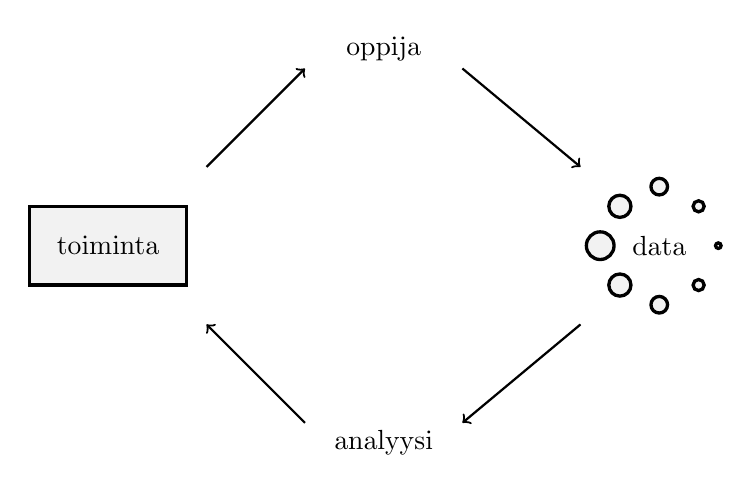
\begin{tikzpicture}
        \filldraw[color=black, fill=black!5, very thick] (-4.5,-0.5) rectangle (-2.5,0.5);

        \filldraw[color=black, fill=black!5, very thick] (4,0.5) circle (2pt);
        \filldraw[color=black, fill=black!5, very thick] (3.5,0.75) circle (3pt);
        \filldraw[color=black, fill=black!5, very thick] (3,0.5) circle (4pt);

        \filldraw[color=black, fill=black!5, very thick] (4,-0.5) circle (2pt);
        \filldraw[color=black, fill=black!5, very thick] (3.5,-0.75) circle (3pt);
        \filldraw[color=black, fill=black!5, very thick] (3,-0.5) circle (4pt);

        \filldraw[color=black, fill=black!5, very thick] (2.75,0) circle (5pt);
        \filldraw[color=black, fill=black!5, very thick] (4.25,0) circle (1pt);

        \node[] at (0,2.5) {oppija};
        \node[] at (3.5,0) {data};
        \node[] at (0,-2.5) {analyysi};
        \node[] at (-3.5,0) {toiminta};


        \draw[thick, ->] (1,2.25) -- (2.5,1.0);
        \draw[thick, ->] (2.5,-1.0) -- (1,-2.25);
        \draw[thick, ->] (-1,-2.25) -- (-2.25,-1);
        \draw[thick, ->] (-2.25,1) -- (-1,2.25);
    \end{tikzpicture}
    \caption{Oppimisanalytiikan eri vaiheet tiivistetysti \citep{clowLearningAnalyticsCycle2012}.}
\end{figure}

Syklissä oppija on oppimisanalytiikan lähtökohta \citep{clowLearningAnalyticsCycle2012}. Oppijoista kerätään dataa analytiikkaa varten, jota koostetaan erilaisista lähteistä \citep{wolffImprovingRetentionPredicting2013}. Oppimisympäristöstä saatavaa dataa voi olla esimerkiksi lokeihin kerätty tieto oppijan oppimisympäristössä liikkumisesta tai opintotietojärjestelmässä aiemmat kurssisuoritukset. Toisaalta myös oppijan oppimiskäyttäytymisen ja -tyylin ymmärtäminen ovat oppimisanalytiikassa keskistä \citep{hasanPredictingStudentPerformance2020}.

Oppijasta muodostunutta dataa voidaan tarkastella ja analysoida oppimisprosessin havainnollistamiseksi \citep{clowLearningAnalyticsCycle2012}. Tämä on oppimisanalytiikan tärkein vaihe. Oppijoista saatavan datan perusteella voidaan tunnistaa esimerkiksi putoamisvaarassa olevia opiskelijoita tai ennustaa heidän menestymistä kurssilla.

Oppimisanalytiikassa syklin viimeisen kohdan, toiminnan, on tarkoitus vaikuttaa oppijaan~\citep{clowLearningAnalyticsCycle2012}. Toimintaa voi olla esimerkiksi oppijan käytössä oleva seurantanäkymä, jossa voi vertailla toisiin opiskelijoihin tai tarvittavan tuen kartoittaminen putoamisvaarassa olevalle opiskelijalle. Oppijan omien havaintojen ja opettajan havaintojen vaikutukset kohdistuvat oppijaan itseensä. Oppija voi hyödyntää analytiikasta saatavaa tietoa oman oppimisensa kehittämiseen hyvin nopeallakin vasteajalla.

Toiminta ei tavoita aina oppijaa, sillä tuloksia voidaan hyödyntää usealla tasolla~\citep{clowLearningAnalyticsCycle2012}. Opettaja voi hyödyntää aiemman kurssi-iteraation kurssiarvosanoja kurssin kehittämisen tukena. Kurssin aikana opettajat toimet voivat vaikuttaa yhden oppijan sijasta myös useampaan oppijaan, ja opettajan toiminnan vaikutukset eivät välttämättä ole heti havaittavissa.

Hallintohenkilöstön toiminnan vaikutukset ovat laajempia ja hitaammin havaittavia heidän yhdistäessä myös opettajalta saatavan palautteen analyysiinsa \citep{clowLearningAnalyticsCycle2012}. Hallintohenkilöstö pystyy toiminnallaan vaikuttamaan isompaan joukkoon oppijoita kuin yksittäinen oppija esimerkiksi jakamalla kurssin kahteen osaan. Toisaalta oppimisanalytiikkaa voidaan hyödyntää laajemmalla tasolla esimerkiksi osana opetussuunnitelmatyötä, jolloin vaikutukset ovat vielä hitaammin havaittavissa, mutta niiden kattavuus on laajin \citep{clowOverviewLearningAnalytics2013}.

Oppimisanalytiikaa voidaan hyödyntää kolmessa eri käyttötarkoituksessa, joita ovat kuvaileva analytiikka, ohjaava analytiikka ja ennustava analytiikka \citep{auvinenOppimisanalytiikkaTuleeOletko2017, danielBigDataAnalytics2015}. Kuvailevassa analytiikassa kuvaillaan ja analysoidaan oppijoista sekä muista oppimisen osa-alueista saatavaa historiatietoa. Kuvaileva analytiikka etsii esimerkiksi nykyisiä oppimistrendejä. Ennustava analytiikka puolestaan tarjoaa oppilaitoksille mahdollisuuden tehdä datan perusteella parempia päätöksiä ja näkymiä nykytilasta. Tavoitteena on estimoida tulevien tapahtumien todennäköisyyksiä. Ohjaava analytiikka puolestaan tarjoaa oppilaitoksille mahdollisuuden arvioida nykyistä toimintaansa vaihtoehtoisten mallien pohjalta ja ohjaa parempiin päätöksiin.
% !TEX root = ./HY-CS-main.tex
\color{black}
\chapter{Datamalli oppijan kehittymisestä\label{datamallioppijankehittymisesta}}

Oppimisanalytiikassa yhdistelemällä tilastollisia menetelmiä ja ennustavaa mallintamista voidaan kohdentaa ohjausta oppijoiden haasteisiin oppimisessa ja tarjoamalla kohdistettua tukea saatavan datan avulla \citep{ranjeethSurveyPredictiveModels2020}. Käytettävät ennustavat mallit voivat olla mitä vain datanlouhinta-, koneoppimis- ja keinoälymenetelmiä. Datalähteenä malleille voidaan hyödyntää eri oppijasta tietoa sisältäviä järjestelmiä, kuten verkko-oppimisympäristö Moodlea. Moodle tarjoaa esimerkiksi aktiviteeteistä laajasti erilaista tietoa hyödynnettäväksi mallin muodostamiseen.

\section{Moodle datalähteenä}

Moodle (Modular Object-Oriented Dynamic Learning System) on vuodesta 1999 lähtien kehittetty avoimen lähdekoodin verkko-oppimisympäristö, joka on julkaistu GPL-3.0 -lisenssillä \citep{dougiamasPowerOpenEducational2021,dougiamasMoodle2022}. Moodlella on yli 315 miljoonaa käyttäjää eri puolilla maailmaa 178 tuhannella eri Moodle-sivustolla \citep{moodle.orgMoodleStatistics}. Moodle on rakennettu käyttäen ohjelmointikielenä PHP:tä ja tiedon tallentamiseen relaatiotietokantaa. Suorat SQL-kyselyt tietokantaan ja Moodlen tarjoamat metodit mahdollistavat Moodlen keräämän tiedon hyödyntämisen osana data-analyysia. Moodlen tietokantarakenteesta löytyy selkeä indeksointi avaimien perusteella \citep{greenMoodle11Database2022}, jonka perusteella tietokantataulusta toiseen asioiden jäljittäminen on mahdollista.

Moodlessa on vakiona 23 erilaista aktiviteettiä, joista jokainen tallentaa erilaista tietoa tietokantaan \citep{dougiamasMoodle2022}. Jokaisella aktiviteetillä on myös omia tietokantatauluja, joihin tallennetaan aktiviteettiin liittyvä tieto. Lisäksi Moodlen kehittäjäyhteisö on julkaissut paljon Moodlea laajentavia aktiveettejä \citep{moodle.orgMoodlePluginsDirectory2022}. Oppilaan osaamista mittaavia aktiviteettejä ovat esimerkiksi tentti, palaute, työpaja, oppitunti, keskustelualue ja H5P. Esimerkiksi työpaja tallentaa kaikki suoritukset tauluun \emph{workshop\_submissions} ja suorituksien arvioinnit tauluun \emph{workshop\_grades} \citep{greenMoodle11Database2022}. Työpaja mahdollistaa myös vertaisarvioinnin (taulussa \emph{workshop\_assessments}), jossa oppija joutuu arvioimaan omaa ja toisten osaamista hyödyntämisen analytiikassa. Keskustelualueelta voidaan mitata oppijoiden aktiivisuutta viestien lukumäärällä \citep{mwalumbweUsingLearningAnalytics2017}. Aktiviteetistä myös saadaan tieto, onko sitä avattu kertaakaan taulun \emph{course\_module\_completion} avulla.

Moodle tallentaa tietokantatauluun \emph{logstore\_standard\_log} kaikki Moodlen Event API:n kautta tulevat tapahtumat \citep{dougiamasMoodle2022, dougiamasLoggingMoodleDocs2021}. Tapahtumien avulla voidaan kerätä tietoa toiminnasta verkko-oppimisympäristössä \citep{agudo-peregrinaCanWePredict2014}. Lokitietoa erilaisista tapahtumista voi esimerkiksi tulla Moodlen ytimen komponenteista, eri aktiviteeteistä, työkaluista ja raporteista riippuen komponentin luonteesta. Useimmat aktiviteetit tallentavat lokiin merkittäviä tapahtumia, kuten suorituksien luomisen aktiviteettiin, kurssimoduulissa vierailun, tenttiin vastaamisen ja vertaisarvioinnin antamisen. Moodlen ytimessä oppijan kannalta tärkeimmät ovat kirjautumiseen ja kurssin katseluun liittyvät tapahtumat. Lokitietoihin tallentuu aina tieto kuka on vieraillut, milloin on vieraillut, missä on vieraillut ja mistä on vieraillut \citep{abdullahLearningStyleClassification2015}. Tapahtumalokin avulla voidaan tarkastella oppijoiden toiminnan painottumista eri kellonaikoihin.

Moodlen yhteisö on myös etsinyt erilaisia tapoja kerätä palautetta oppijoilta. Yksi tälläinen on pikapalautetoiminnallisuus (block\_point\_view), joka antaa kolmiportaisen itsearviointimahdollisuuden aktiviteettikohtaisesti \citep{fombaronMoodlePluginPoint2021}. Tämä mahdollistaa helpon ja nopean tavan saada oppijalta itsearviointidataa siitä, miten oppija itse näkee oman suoriutumisensa kyseisessä tehtävässä. Tietokantataulusta \emph{block\_point\_view} pystytään hakemaan käyttäjän äänestystulos kurssin, kurssimoduulin tai käyttäjän perusteella.

Joidenkin tietojen, kuten oppijan tarkemman toiminnan seuraamiseen sivulla tarvitaan kolmannen osapuolen tuottamaa tekniikkaa \citep{filvaGoogleAnalyticsTime2014}. Tälläinen seuraamiseen soveltuva työkalu on esimerkiksi Google Analytics, joka seuraa tarkemmin käyttäjän toimintaa sivustolla. Moodlen lokitiedoista selviää milloin sivu on ladattu, mutta tietoa kuinka kauan oppija sivulla on todellisuudessa viettänyt aikaa ei tällä menetelmällä saada \citep{dougiamasMoodle2022}. On teoreettisesti mahdollista, että oppija on avattuaan sivun katsellut sitä minuutin ajan ja tämän jälkeen lähtenyt kahville. Jos seuraava sivulataus on tunnin päästä, niin tästä ei pystytä luotettavasti laskemaan sivulla vietettyä todellista aikaa.

\color{blue}
Learning Analytics API tarjoaa Moodlen oman rajapinnan oppimisanalytiikan toteuttamiseen \citep{oliveSupervisedLearningFramework2018}. Moodlessa se jakautuu kahteen osaan, Moodlen Analytics API:n ja Machine Learning backendiin. Analytics API tuottaa mallien tarvitsemaa tietoa koneluettavassa CSV-muodossa. Backend puolestaan vastaa itse tiedon käsittelystä ja analysoinnista. Tämä mahdollistaa oppimisanalytiikkamallien integroimisen osaksi Moodlea helposti.
\color{black}

\section{Yleistetty malli}
\color{red}
tilastollinen malli kuvaa optimia, ja verrataan kuinka data sopii tähän malliin
\color{black}

% Linear regressionista hyvää tietoa \citep{rossIntroductoryStatistics2017} - Ch 12 \\
% Naive Bayessian Ch 16
Datamallin rakentaminen on iteratiivinen prosessi, jossa on useita vaiheita \citep{hamalainenClassifiersEducationalData2010}. Iteratiivisen prosessin aikana kokeillaan useita erilaisia malleja, datan esitysmuotoja ja algoritmien asetuksia löytääksemme parhaan mahdollisen datamallin. Valitun mallin toimivuus voidaan todentaa luokittelun onnistumisella, sillä mallin soveltuvuus voidaan kyseenalaistaa liian monen luokitteluvirheen jälkeen.

% HOX TÄÄ TARVII UUDELLEENKIRJOITUSTA, MUTTA MITEN!?
Oppimisanalytiikassa usein käytetään luokittelua, jota hyödynnetään opetuksessa yleisesti opettajien arvioidessa oppijoiden tietotasoa, motivaatiota ja käytöstä \citep{hamalainenClassifiersEducationalData2010}. Oppimisanalytiikassa luokittelua tehdään selitettävän muuttujan arvoa ennustavalla mallilla, jota ennustetaan selittävien muuttujien arvojen avulla. Luokittimia voidaan tehdä joko ammattilaisten käsityönä tai nykyisin yleisemmällä tavalla opettaa luokitin luokittelemaan olemassa olevalla datalla.

Useissa oppimisanalytiikkaa käsittelevissä tutkimuksissa on kokeiltu erilaisia luokittelualgoritmejä parhaiten toimivan mallin löytämiseksi \citep{akcapinarUsingLearningAnalytics2019}. Usein käytettyjä algoritmejä ovat naiivi Bayes, Classification Tree, Random Forest, tukivektorikone (SVM), neuroverkko, CN2 rules ja k-lähinaapurimenetelmä. Yksi tapa etsiä parhaiten toimivaa mallia on tehdä suorituskykymittauksia, joissa tarkastellaan tarkkuutta, herkkyyttä, yksityiskohtaisuutta ja F-Measurea.

Yksi tapa tehdä luokittelua on käyttää naiivia Bayesin luokitinta \citep{natinggaDataScienceAlgorithms2018}. Naiivi Bayesin luokitin pohjautuu Bayesin teoreemaan $$P(A | B) = \frac{P(B | A) \cdot P(A)}{P(B)},$$ missä $A$ ja $B$ ovat tapahtumia, $P(A)$ on todennäköisyys tapahtumalle $A$ olla tosi ja $P(A | B)$ on ehdollinen todennäköisyys tapahtumalle $A$ olla tosi, mikäli tapahtuma $B$ on tosi. Naiivissa Bayesin luokittimessa datapisteiden joukolle annetaan Bayesin teoreeman perusteella todennäköisin luokka. Tämä tapahtuu laskemalla todennäköisyys sille, kuinka todennäköisesti asia A tapahtuu, jos ehto B saa tietyn arvon.

Bayesin teoreemaa voidaan hyödyntää myös useamman todennäköisyystapahtuman kanssa, jolloin käytetään laajennettua Bayesin teoreemaa \citep{natinggaDataScienceAlgorithms2018}. Jos määritellään tapahtumat $B_1, \ldots, B_n$ olemaan ehdollisesti riippumattomia tapahtumasta $A$, niin Bayesin teoreema voidaan esittää muodossa $$P(A | B_1, \ldots, B_n) = \frac{P(B_1, \ldots, B_n | A) \cdot P(A)}{P(B_1, \ldots, B_n)}.$$ Nämä satunnaismuuttujina toimivat todennäköisyystapahtumat voivat olla diskreettejä tai jatkuvia seuraten todennäköisyysjakaumaa, kuten normaalijakaumaa.

Käytettäessä Bayesilaista todennäköisyyttä täytyy vertailtavien tapahtumien olla riippumattomia toisistaan \citep{natinggaDataScienceAlgorithms2018}. Jos vertaillaan lämpötilaa ja vuodenaikaa keskenään, niin näiden välillä havaitaan olevan riippuvuus: talvella on kylmää ja kesällä lämmintä. Tämä estää Bayesin teoreeman käyttämisen luokittelemiseen. Tämä voidaan kiertää tekemällä analyysia niille data-aineiston tapahtumille, jotka eivät ole riippuvia toisistaan.

Toinen mahdollisuus tehdä tilastollista analyysia kerätylle oppimisdatalle on regressioanalyysi \citep{songLearningAnalyticsEducational2018, romeroEducationalDataMining2010, papamitsiouLearningAnalyticsEducational2014}. Regressioanalyysiä voidaan tehdä usealla eri tavalla, kuten yksinkertaisella lineaarisella regressiolla, usean selittäjän lineaarisella regressiolla ja logistisella regressiolla. Regression avulla voidaan ennustaa lineaarisesti esimerkiksi kuinka opiskelija tulee menestymään eri selittävien muuttujien vaikutus huomioiden.

Lineaarinen regressio kuvaa yhden selittävän ja yhden selitettävän muuttujan yhteyttä toisiinsa \citep{rossIntroductoryStatistics2017}. Yksinkertainen lineaarinen regressio voidaan esittää kaavana $$Y = \alpha + \beta x + e,$$ jossa $x$ kuvaa selittävää muuttujaa ja $y$ kuvaa selitettävää muuttujaa. Parametrit $\alpha$ ja $\beta$ ovat tuntemattomia suureita, estimaattoreita, jotka estimoidaan datan perusteella. Muuttuja $e$ kuvaa satunnaista virhettä, jonka oletetaan noudattavan normaalijakaumaa odotusarvolla $0$ ja varianssilla $\sigma^2$. Varianssin oletetaan olevan sama riippumatta selittävistä muuttujista $x$.

Parametrien $\alpha$ ja $\beta$ estimointiin voidaan käyttää pienimmän neliösumman estimointia \citep{rossIntroductoryStatistics2017}. Tällöin halutaan löytää sellaiset arvot estimaateille $\alpha$ ja $\beta$, joilla virheen neliösumma $\sum^n_{i=1} \epsilon^2_i$ on mahdollisimman pieni. Pienimmän neliösumman estimaatit $\hat{\alpha}$ ja $\hat{\beta}$ parametreille $\alpha$ ja $\beta$ saadaan laskettua kaavoista $$\hat{\beta} = \frac{\sum^n_{i=1}(x_i - \overline{x})(Y_i - \overline{Y})}{\sum^n_{i=1}(x_i - \overline{x})^2}$$ ja $$\hat{\alpha} = \overline{Y} - \hat{\beta}\overline{x},$$ missä $\overline{x} = \frac{\sum^n_{i=1}x_i}{n}$ ja $\overline{Y} = \frac{\sum^n_{i=1}Y_i}{n}$.

Estimoidussa regressioviivassa $y = \hat{\alpha} + \hat{\beta}x$ estimaatti $\hat{\alpha}$ kuvaa suoran kulmakerrointa ja estimaatti $\hat{\beta}$ suoran vakiota, eli kohtaa y-akselilta missä suora leikkaa y-akselin \citep{rossIntroductoryStatistics2017}. Tämän estimoidun regressioviivan avulla voidaan ennustaa selitettävän muuttujan $y$ arvoja käyttäen selittävän muuttujan x arvoja.

Yksinkertainen lineaarinen regressio voidaan laajentaa usean selittäjän lineaariseksi regressioksi, joka kuvaa useamman selittävän muuttujan $x_1, \ldots, x_i$ vaikutusta selitettävään muuttujaan $Y$ \citep{rossIntroductoryStatistics2017}. Matemaattisena kaavana esitettynä usean selittäjän lineaarinen regressio on $$Y = \beta_0 + \beta_1x_1 + \beta_2x_2 + \ldots + \beta_kx_k + e,$$ jossa $Y$ on selitettävä muuttuja, ja $x_i$ kuvaa selittäviä muuttujia, missä $i = 1, \cdots, k$. Regressioparametrejä yhtälössä kuvaa $\beta_0, \beta_1, \cdots, \beta_k$ ja satunnaisvirhettä $e$.

Myös regressiossa täytyy selittävien muuttujien olla riippumattomia toisistaan, eli nämä muuttujat eivät saa olla keskenään korreloivia \citep{daoudMulticollinearityRegressionAnalysis2017}. Tätä ilmiötä kutsutaan multikollineaarisuudeksi. Ilmiö voidaan havaita tapauksissa, joissa tapahtuu suurta vaihtelua estimoiduissa kertoimissa lisättäessä tai poistettaessa selittäviä muuttujia tai poistettaessa yksittäisiä datapisteitä.

\section{Datamallin rakentamisessa huomioitavaa}
\color{blue}
Ennen datan syöttämistä analysointia tai luokittelua tekevälle mallille, tulee aineistolle suorittaa esikäsittely \citep{romeroSurveyPreProcessingEducational2014}. Esikäsittely aloitetaan keräämällä tarvittava data, joka ryhmitellään sopiviin ja järkeviin kokonaisuuksiin. Datan ryhmittelyn jälkeen poistetaan siitä kaikki epäolennainen ja virheellinen sisältö.
Aineistosta tunnistetaan käyttäjät ja heidän asiointisessiot kohdistaaksemme analyysin oikeisiin oppijoihin.
Korreloivat ja toisteiset muuttujat jätetään pois, kun valitaan aineistosta sopivat selittävät muuttujat. Isoista data-aineistoista poistetaan aiempien vaiheiden jälkeen turhiksi jääneet kentät, jotka olisivat epäolennaisia prosessille. Lopuksi tarkastellaan mahdollisuutta muodostaa uusia muuttujia olemassa olevien muuttujien perusteella, kuten normalisoida jonkin muuttujan arvot tietylle välille tai muuttaa esitystapaa sopivammaksi.

Yhdistelläksemme tietyllä välillä liikkuvia muuttujia kategoristen muuttujien kanssa, voidaan käyttää dummy-muuttujia kuvaamaan näitä arvoja \citep{rossIntroductoryStatistics2017}. Tällöin voidaan hyödyntämään sellaisia selittäviä kategorisia muuttujia, jotka eivät lähtökohtaisesti ole numeerisessa muodossa. Jos esimerkiksi usean selittäjän lineaarisessa regressiossa muuttuja $x_3$ kuvaa onko oppija tutkinto-opiskelija, voidaan tämä esittää numeraalisessa muodossa seuraavasti: $$x_3 = \begin{cases}1 = \text{oppija on tutkinto-opiskelija} \\ 0 = \text{oppija ei ole tutkinto-opiskelija}\end{cases}.$$

Mallia toteutettaessa on huomioitava yli- ja alisovittamisen vaara, jotta mallin tarkkuus ei kärsisi \citep{hamalainenClassifiersEducationalData2010}. Ylisovittamisessa malli on sovitettu koulutusaineistoon niin tarkasti, että se huomioi jopa kaikki erikoistapaukset sekä koulutusdatan virheet. Tämä ilmenee liian monimutkaisena mallina suhteessa käytettävän data-aineiston kokoon. Alisovittamisessa liian yksinkertainen malli ei pysty välttämättä tulkitsemaan data-aineistoa ja täten malli ei kuvaa todellisuutta tai kuvaa sitä todella vähän.

Yksi tapa jakaa data-aineisto koulutus- ja testidataan on käyttää ristivalidointia, kuten k-kertaista ristiinvalidointia \citep{deisenrothMathematicsMachineLearning2020}. Aineisto jaetaan $k$ osaan, joista yhtä osaa kerrallaan käytetään testiaineistona $\mathcal{V}$ ja $k-1$ osaa koulutusaineistona $\mathcal{R}$. Tällöin aineistosta käytetään suurin osa mallin kouluttamiseen, mutta samasta aineistosta saadaan myös testiaineisto muodostettua. Ristiinvalidoinnissa käydään läpi kaikki mahdolliset $k$ vaihtoehtoa valita testiaineisto jakamalla data-aineisto kahteen osaan $D = \mathcal{R} \cup \mathcal{V}$, missä $\mathcal{R} \cap \mathcal{V} = \emptyset$. Näiden $k$-suorituskerran muodostamien mallien suorituskyky tarkastellaan keskiarvona.

\begin{figure}[h]
    \centering
    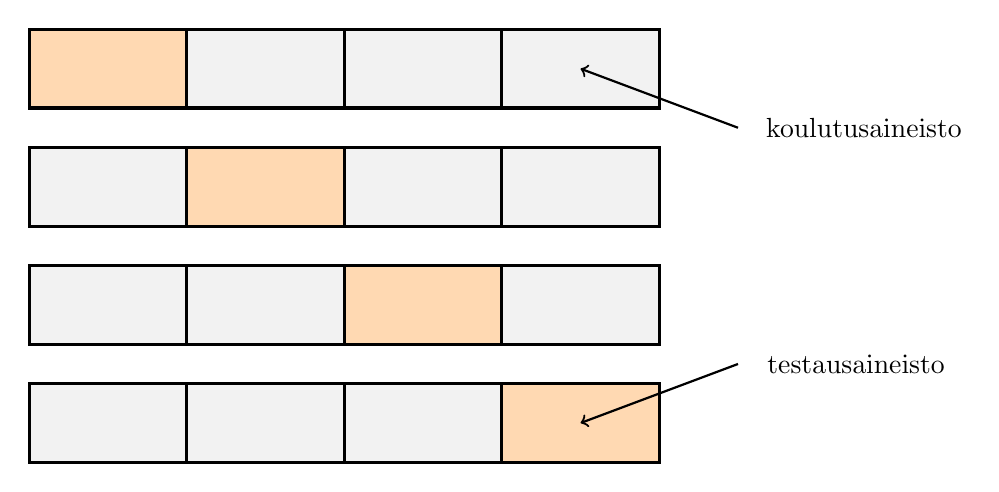
\begin{tikzpicture}
        \filldraw[color=black, fill=black!5, very thick] (0,0) rectangle (2,1);
        \filldraw[color=black, fill=black!5, very thick] (2,0) rectangle (4,1);
        \filldraw[color=black, fill=black!5, very thick] (4,0) rectangle (6,1);
        \filldraw[color=black, fill=orange!30, very thick] (6,0) rectangle (8,1);

        \filldraw[color=black, fill=black!5, very thick] (0,1.5) rectangle (2,2.5);
        \filldraw[color=black, fill=black!5, very thick] (2,1.5) rectangle (4,2.5);
        \filldraw[color=black, fill=orange!30, very thick] (4,1.5) rectangle (6,2.5);
        \filldraw[color=black, fill=black!5, very thick] (6,1.5) rectangle (8,2.5);

        \filldraw[color=black, fill=black!5, very thick] (0,3) rectangle (2,4);
        \filldraw[color=black, fill=orange!30, very thick] (2,3) rectangle (4,4);
        \filldraw[color=black, fill=black!5, very thick] (4,3) rectangle (6,4);
        \filldraw[color=black, fill=black!5, very thick] (6,3) rectangle (8,4);

        \filldraw[color=black, fill=orange!30, very thick] (0,4.5) rectangle (2,5.5);
        \filldraw[color=black, fill=black!5, very thick] (2,4.5) rectangle (4,5.5);
        \filldraw[color=black, fill=black!5, very thick] (4,4.5) rectangle (6,5.5);
        \filldraw[color=black, fill=black!5, very thick] (6,4.5) rectangle (8,5.5);

        \draw[thick, ->] (9,1.25) -- (7,0.5);
        \node[] at (10.5,1.25) {testausaineisto};

        \draw[thick, ->] (9,4.25) -- (7,5);
        \node[] at (10.6,4.25) {koulutusaineisto};
    \end{tikzpicture}
    \caption{Ristiinvalidoinnissa data-aineisto jaetaan kerrallaan $k$ osaan, missä $k-1$ osaa ovat koulutusaineistoa (harmaalla merkityt osuudet) ja yksi osa testausaineistoa (oranssilla merkitty osuus) \citep{deisenrothMathematicsMachineLearning2020}.}
\end{figure}

Koulutusaineistolla $\mathcal{R}$ koulutetun mallin $f$ suorituskykyä tarkastellaan testausaineiston $\mathcal{V}$ avulla, jolle lasketaan keskineliövirheen neliöjuuren avulla empiirinen riski testausaineistolla $\mathcal{V}$ \citep{deisenrothMathematicsMachineLearning2020}. K-kertaisessa ristiinvalidoinnissa lasketaan jokaiselle koulutusaineiston $k$-osan $\mathcal{R}^{(k)}$ predikaattorille $f^{(k)}$ empiirinen riski $R(f^{(k)}, \mathcal{V}^{(k)})$ käyttäen testiaineistoa $\mathcal{V}^{(k)}$. Kaikille mahdollisille $k$-osaan jaoille ristiinvalidointi arvioi odotetun yleistysvirheen kaavasta $$\mathds{E}_{\mathcal{V}}[R(f,\mathcal{V})] \approx \frac{1}{K}\sum^{K}_{k=1} R(f^{(k)}, \mathcal{V}^{(k)}).$$ Käytettävässä arvioinnissa on kaksi lähdettä, joista toisessa rajatulla koulutusaineistolla ei välttämättä saada parasta mahdollista $f^{(k)}$ ja toisessa testausaineistolla ei saada tarkkaa arviota riskistä $R(f^{(k)}, \mathcal{V}^{(k)})$.

\color{black}

% \color{red}
% Useiden eri mallien välisessä vertailussa naiivi Bayes oli ennustustamisen osalta paras algoritmi \citep{kotsiantisPREDICTINGSTUDENTSPERFORMANCE2004}.
% \color{black}
% !TEX root = ./HY-CS-main.tex
\chapter{Datamallin hyödyntäminen oppimisanalytiikassa\label{hyodyntaminen}}

Oppimisanalytiikkaa voidaan hyödyntää usealla eri tasolla \citep{longPenetratingFogAnalytics2011,siemensLearningAnalyticsEmergence2013}. Kurssitasolla voidaan seurata opiskelijan toimintaa kurssilla ja tehdä havaintoja kurssin edistymisestä sekä sillä menestymisestä. Tätä voidaan tehdä esimerkiksi luokittelulla tai ennustavilla malleilla.
% Yksi taso on hyödyntää oppimisanalytiikkaa sisällön suosittelemiseen. Tässä oppijan oppimispolku muotoillaan osaamista vastaavaksi esimerkiksi ohjaamalla perusasiat jo hyvin osaava oppija haasteellisemmalle kurssille tai tarjotaan heikommin pärjäävälle opiskelijalle taitotasoa vastaavia tehtäviä. \color{red}(HOX! Tsiikaa noi muut kolme muuta Longin nostoa sekä table 1 + synkronoi seuraaviin kappaleisiin. Muotoile seuraavat kappaleet Longin tasoajattelun kanssa.)\color{black}
Ennustavien mallien avulla muodostetaan keskimääräistä oppijaa kuvaavia malleja, joiden avulla yksittäisiä oppijoita voidaan vertailla \citep{wolffImprovingRetentionPredicting2013}.
%Ennustavan mallinnuksen avulla voidaan ennustaa esimerkiksi kuinka oppija tulee menestymään kurssilla ja onko oppija pääsemässä kurssia läpi. Tämä tapahtuu vertailemalla oppijaa muodostettuun malliin ja ennusteen perusteella katsotaan onko oppija vaarassa olla läpäisemättä kurssia.

\section{Yksitäiseen oppijaan kohdennetut ehdotukset}

% Multiple linear regressio \citep{agudo-peregrinaCanWePredict2014} \\
% Linear regression \citep{tempelaarSearchMostInformative2015} \\
% Logistic regression \citep{barberCourseCorrectionUsing2012} \\
% Logistic regression \citep{garmanLogisticApproachPredicting2010} \\
% Naïve Bayes algorithm \citep{barberCourseCorrectionUsing2012} \\
% Decision tree \citep{wolffImprovingRetentionPredicting2013} \\

Oppijan menestymistä kurssilla voidaan ennustaa eri tarkoituksissa \citep{barberCourseCorrectionUsing2012a}. Tähän voidaan hyödyntää aiempien kurssien menestystietoa muista lähteistä, sekä kurssin edistyessä lisätä kurssisuorituksista saatavaa tietoa mukaan analyysiin. Yhdistämällä tämän visualisointiin, voidaan tarjota oppijalle reaaliaikainen näkymä kurssiarvosanasta ja hyödyntää tätä motivaattorina. Yksi ennustamisen mahdollisuus on tarkastella valmistuuko koulutukseen hakija ennusteen mukaan tavoiteaikataulussa.

Toisaalta voidaan tarkastella onko oppija vaarassa pudota kurssilta \citep{oliveSupervisedLearningFramework2018, suhonenUsingMoodleData2019}. Tarkastellaan oppijan toimintaa verkko-oppimisympäristössä ja yritetään löytää eri merkkejä oppijan putoamisesta kurssilta. Tarkastelua voidaan laajentaa eri kurssien väliseksi \citep{kinnari-korpelaOppimisanalytiikallaTehokkaampaanOhjaukseen2020} ja analytiikan löytäessä putoamisvaarassa olevan oppijan, voidaan hänelle tarjota kohdistetusti tukea oppimiseen jo aikaisessa vaiheessa. Moodleen on sisäänrakennettu Learning Analytics API:n avulla opiskelijoiden tippumisen tunnistamisen tarjoava malli sekä kurssin opetuksen puuttumisen tunnistava malli \citep{oliveSupervisedLearningFramework2018,monllaoAnalyticsAPIMoodleDocs2021}. \color{red} Avaa Moodle osuutta vielä tarkemmin. \color{black}
% Etsi tämän lähde jostain: Paras tapa tunnistaa oppijan mahdollinen putoaminen on vertailla oppijan aiempaan käyttäytymiseen ja tunnistaa muutoksen merkkejä siinä (tälle oli kiva lähde, löytynee luvusta 3 :D).

Naiivilla Bayesin luokittimella voidaan esimerkiksi yrittää tunnistaa opiskelijoita, jotka ovat vaarassa saada hylätyn osallistumaltaan kurssilta \citep{barberCourseCorrectionUsing2012}. Selittävinä muuttujina oli henkilöön liittyviä taustatietoja, suoritettujen opintopisteiden suhde yritettyihin opintopisteisiin sekä toimintaa verkko-oppimisympäristön keskustelualueella. Selittäville muuttujille oli annettu eri painoarvoja riippuen kurssin viikosta.
% Verrattuna logistiseen regressioon, lisättyjen selittävien muuttujien kanssa nähtiin kurssin viikolla 0 35 \%-yksikön parannus ennustustarkkuudessa datamäärän ollessa pienempi ja eron kaventuessa huomattavasti lähemmäs toisiaan viikolla 3 datamäärän kasvettua, missä logistisella regressiolla keskimäärin 94\% ennustuksista onnistui ja naiivilla Bayesillä 95\% onnistui.

Usean selittäjän lineaarista regressiota voidaan hyödyntää esimerkiksi etsittäessä eri relaatioita opiskelijan verkko-oppimisympäristön toiminnan ja akateemisen menestyksen väliltä \citep{agudo-peregrinaCanWePredict2014}. Riippumattomia selittäviä muuttujia olivat eri tyyppiset interaktiot verkko-oppimisympäristössä ja riippuvana selittävänä muuttujana jokaisen oppijan saamana kurssin päättöarvosanana esittety akateeminen menestys, joiden väliltä löydettiin merkittäviä relaatioita.

Oppimispolku on ohjeistus, joka kertoo oppimistehtävien ohjeistukset ja tavoitteet, sekä havainnollistaa oppimisen edistymistä kurssin aikana \citep{toivolaFlippedLearningKaanteinen2017}. Oppimispolun halutaan mahdollistaa oppijan oman luontaisen oppimistahdin hyödyntäminen. Oppimisanalytiikan avulla voidaan visualisoida oppijan edistyminen oppimispolulla ja tarjota myös suosituksia seuraavista tehtävistä \citep{longPenetratingFogAnalytics2011}. Jos oppija ei ole vielä ymmärtänyt jotain oppimispolun osa-aluetta, voi analytiikka ehdottaa lisätehtävää osaamisen vahvistamiseksi ennen seuraavaan osa-alueeseen siirtymistä. Pikapalautetta voidaan hyödyntää itsearvioiden toteuttamiseen ja edelleen analytiikan tukena.

Tätä voitaisiin myös hyödyntää kurssipolkujen suunnittelussa ehdottamalla esimerkiksi oppijalle seuraavia kursseja aiempien kurssien menestyksen pohjalta \citep{longPenetratingFogAnalytics2011}. Jos oppija ei ole esimerkiksi pärjännyt matriisilaskennan ensimmäisellä kurssilla, niin oppimisanalytiikka voisi ehdottaa matriisilaskennan ensimmäisen kurssin asioita kertaavaa kurssia ennen siirtymistä toiselle kurssille.

\section{Opetuksen kehittämiseen kohdennetut ehdotukset}

Oppimisanalytiikan avulla voidaan tehdä opetuksen kehttämistä \citep{romeroEducationalDataMining2010}. Oppimisanalytiikasta saatavalla datalla voidaan suunnitella kurssien resursointia, kehittää opetussuunnitelmia sekä tukea hallinnon päätöksiä. Oppimisanalytiikalla voidaan löytää nykyisistä kursseista heikkoja kohtia, joihin ratkaisu voi olla esimerkiksi uuden kurssin luominen tai nykyisen kehittäminen tukemaan osaamisvajeen paikkaamista. Tämä voi näkyä esimerkiksi oppimateriaalin kehittämisenä, mikäli analytiikka osoittaa tietyn osa-alueen tehtävien menevän muita heikommin, kun saman aikaisesti tiettyä opetusmateriaalin osaa tarkastellaan muita enemmän.

\color{red} Moodlen ei opetusta kurssilla malli tähän. Lihavoita lukua. \color{black}

\color{red}
\section{Ehdotuksien tulkinnan rajoitteet}

\begin{enumerate}
    \item etiikka?! \citep{kailaEthicalConsiderationsLearning2019}
    \item laki, henkilötieto? \citep{hannulaOppijanDigitaalinenJalanjalki2017}
    \item virhearviot ja model bias
    \item mallien ennustuksien paikkaapitävyyden todennäköisyydet - kuinka todennäköisesti ennustuksen tulos pitää paikkansa. voidaanko 72 prosentin todennäköisyyttä pitää sellaisena, että se toimii luotettavana ohjauksen työkaluna?
\end{enumerate}
% !TEX root = ./HY-CS-main.tex
\chapter{Yhteenveto\label{yhteenveto}}

Oppimisanalytiikkaa voidaan kuvata oppijoista kerättävän tietoaineiston mittaamisena, keräämisenä, analysointina ja raportointina \citep{siemensLearningAnalyticsEmergence2013,clowLearningAnalyticsCycle2012}. Tätä hyödynnetään oppimisen ja sen ympäristön ymmärtämiseen sekä optimoimiseen.

Oppimisanalytiikkaa voidaan yleensä kuvata neljän osa-alueen syklinä: oppija, data, analyysi ja toiminta \citep{clowLearningAnalyticsCycle2012}. Oppimisanalytiikan lähtökohta on oppija, joka tuottaa oppimisanalytiikassa käytettävän datan \citep{wolffImprovingRetentionPredicting2013}. Kerättävä data voi olla esimerkiksi oppimisympäristöistä. Kerätyn datan pohjalta voidaan tarkastella ja analysoida oppimisprosessin havainnollistamiseksi, joka on oppimisanalytiikan tärkein vaihe. Toiminnan avulla on tarkoitus vaikuttaa oppijaan ja tarjota mahdollisuuksia kehittää omaa oppimistaan.

Oppimisanalytiikassa tuloksien hyödyntäjiä voi olla useita, eikä toiminta vältämättä tavoita aina oppijaa \citep{clowLearningAnalyticsCycle2012}. Oppimisanalytiikasta saatavia tietoja voidaan hyödyntää oppijan toiminnan kehittämisen lisäksi opettajan toiminnan kehittämiseen, hallintohenkilöstötasolla esimerkiksi kohdistettaessa resursseja tai vielä laajemmalla tasolla esimerkiksi osana opetussuunnitelmatyötä \citep{clowOverviewLearningAnalytics2013}. Tällöin voidaan havaita, että oppimisanalytiikka voi vaikuttaa sekä yhden tietyn oppijan toimintaan, mutta laajemmin myös useiden oppijoiden toiminnan kehittämiseen. Kehittämällä raportointia kohti enemmän datalla johtamista, pystytään tukemaan oppijoita oppimisanalytiikalla saavuttamaan tavoitteitaan paremmin.

Tilastollisten mallien sekä ennustavan mallintamisen avulla voidaan oppimisanalytiikan avulla tarjota ohjausta oppijoiden oppimishaasteisiin sekä tarjota kohdistettua tukea tietoaineiston avulla \citep{ranjeethSurveyPredictiveModels2020}. Eri oppijan tietoa sisältävistä järjestelmistä, kuten Moodelsta saatavaa tietoaineistoa voidaan käsitellä eri datanlouhinta-, koneoppimis- ja keinoälymenetelmillä.

Yksi esimerkki oppimisanalytiikan tietoaineiston lähteeksi on Moodle. Moodle on avoimen lähdekoodin verkko-oppimisympäristö, jolla on yli 315 miljoonaa käyttäjää eri puolilla maailmaa \citep{dougiamasPowerOpenEducational2021,dougiamasMoodle2022,moodle.orgMoodleStatistics}. Moodle tarjoaa useita erilaisia aktiviteettejä, jotka tallentavat tietoa oppijan toiminnasta relaatiotietokantaan. Oppimisanalytiikan osalta tentti, palaute, työpaja, oppitunti, keskustelualue ja H5P tuottaa konkreettista tietoa oppijan suoritumisesta. Moodlen tapahtumalokiin Event API:n kautta tallennetut tapahtumat tuottavat oppijan toiminnan kannalta merkittävää tietoaineistoa esimerkiksi tehtävien avauskertojen sekä oppijan toiminnan ajoittumisen osalta \citep{dougiamasLoggingMoodleDocs2021, abdullahLearningStyleClassification2015}.

Järjestelmistä saatavaa tietoaineistoa voidaan käsitellä ennustaviin malleihin pohjautuvilla luokittimilla \citep{hamalainenClassifiersEducationalData2010}. Bayesin teoreemalla voidaan laskea todennäköisyystapahtumien avulla kunika todennäköisesti jokin asia A tapahtuu, mikäli ehto B saa tietyn arvon \citep{natinggaDataScienceAlgorithms2018}. Toinen mahdollinen ennustava malli on käyttää regressioanalyysiä, kuten lineaarista regressiota \citep{rossIntroductoryStatistics2017}. Se kuvaa yhden selitettävän ja yhden tai useamman selittävän muuttujan välistä yhteyttä toisiinsa.

Valmisteltaessa tietomallia on huomioitava myös aineiston käsitteleminen ennen sen syöttämistä ennustavalle mallille \citep{romeroSurveyPreProcessingEducational2014, rossIntroductoryStatistics2017}. Esikäsittelyssä kerätään kaikki tarvittava tietoaineisto ja tämän jälkeen tietoaineistoa ryhmitellään, siistitään ja muokataan analyysiin sopivaan muotoon. Lisäksi tarkastellaan mahdollisten tekomuuttujien tarve.

Oppimisanalytiikan avulla voidaan kohdentaa ehdotuksia yksittäisiin oppijoihin esimerkiksi tunnistamalla mahdollisesti kurssin reputtavia oppijoita \citep{barberCourseCorrectionUsing2012} sekä etsimällä relaatioita oppijoiden verkko-oppmisympäristön toiminnan ja akateemisen menestyksen väliltä \citep{agudo-peregrinaCanWePredict2014}. Myös koko koulupolkua voidaan tarkastella ennustamalla valmistuuko koulutukseen hakija tavoiteaikataulussa \citep{barberCourseCorrectionUsing2012a}.

Opetuksen kehittämiseen voidaan oppimisanalytiikkaa soveltaa esimerkiksi kehittämällä resurssien sijoittelua ja käyttöä \citep{longPenetratingFogAnalytics2011, romeroEducationalDataMining2010}. Käytännössä voidaan hyödyntää esimerkiksi kurssien heikkojen kohtien, oppilaitoksen onnistumisien ja haasteiden löytämiseen sekä opetussuunnitelmien sekä hallinnon päätöksien tukemiseen. Näiden avulla voidaan kohdistaa resurssit vastaamaan todellista tarvetta sekä tarkastelemaan onko jollekin osa-alueelle kohdistettava enemmän opetusresursseja.

Oppimisanalytiikalla ei voida korvata oppijoiden ohjausta, vaan oppimisanalytiikka on yksi työkalu kaikkien muiden työkalujen joukossa \citep{auvinenOppimisanalytiikkaTuleeOletko2017}. Oppimisanalytiikalla voidaan tehostaa tätä toimintaa. Se tulee ymmärtää työvälineenä, jonka avulla ymmärretään paremmin oppimista ilmiönä ja havainnollistaa mitä oppimisessa tapahtuu. Oppijan on helpompi ymmärtää oppimisessa olevia haasteita, kun ne pystytään esittämään paljon konkreettisemmin.


%%%%%%%%%%%%%%%%%%%%%%%%%%%%%%%%%%%%%%%%%%%%%%%%%%%%%%%%%
%\cleardoublepage                          %fixes the position of bibliography in bookmarks
%\phantomsection
\addcontentsline{toc}{chapter}{\bibname}  % This lines adds the bibliography to the ToC
\printbibliography

%%%%%%%%%%%%%%%%%%%%%%%%%%%%%%%%%%%%%%%%%%%%%%%%%%%%%%%%%
\backmatter
\begin{appendices}

%% A sample Appendix

\appendix{Tekoälyn käyttö tutkielmassa\label{appendix:tekoalynkaytto}}

Tekoälyä ei ole käytetty osana tutkielmaprosessia.

%% another appendix
%% 
\appendix{Instructions for LaTex}

\section{General Setup}

In the HY-CS-main.tex file you will find the following STEPS 0--5. Below you can find related instructions.
\vspace{0.5cm}

\textbf{STEP 0 -- Access the thesis template}

\begin{itemize}
\item Import the thesis template into a new Overleaf project. The easiest way to do it is to:
\begin{itemize}
    \item Obtain a zip file of the LaTeX template from the webpage of your programme.
    \item Go to \url{https://www.overleaf.com/edu/helsinki} and login to Overleaf with your university credentials.
    \item Go to the list of your projects at \url{https://www.overleaf.com/project}, click ``New Project'' and ``Upload Project''.,  the projects under your account
    \item Then upload the zip with the template.
    \item You are now ready to write your thesis in Overleaf by editing the template, you can start by renaming the project.
\end{itemize}
\end{itemize}


{\textbf{STEP 1 -- BSc or MSc thesis?}}
\begin{enumerate}
\item Select whether your are writing BSc (tkt) or MSc (csm for CS) thesis.
\item Select your language: \texttt{finnish}, \texttt{english}, or \texttt{swedish}.
\item If you are writing MSc select your line / track.
\end{enumerate}


{\textbf{STEP 2 -- Set up your personal information}}

\begin{enumerate}
\item Specify the title of your thesis with \texttt{\textbackslash title\{\}}.
\item Specify your name to the author field with \texttt{\textbackslash author\{\}}.
\item Specify the names of your supervisors of the thesis with \texttt{\textbackslash supervisors\{\}}.
\item Specify the keywords of the thesis with \texttt{\textbackslash keywords\{\}}.
\item Specify the ACM classification terms of the thesis with \texttt{\textbackslash classification\{\}}. See \url{https://dl.acm.org/ccs} for more information.
\end{enumerate}

{\textbf{STEP 3 -- Write your abstract}}

\begin{itemize}
\item You can have the abstract in multiple languages with the \texttt{otherlanguages} environment. The example below shows how to provide an English abstract:

\begin{verbatim}
\begin{otherlanguage}{english}
\begin{abstract}
Your abstract text goes here.
\end{abstract}
\end{otherlanguage}
\end{verbatim}

\end{itemize}

{\textbf{STEP 4 -- Writing your thesis}}

\begin{enumerate}
\item There are some minimal contents and instructions below
\item Remove, or comment out, this appendix from your thesis.
\end{enumerate}

{\textbf{STEP 5 -- Set your bibliography style}}

\begin{itemize}
\item The default is Author-Year style (Einstein, 1905), but it can be easily changed to numbered [1] or alphabetical [Ein05] , as the examples of these are in comments.
\item Discuss the style to use with your supervisor.
\end{itemize}

\section{Bibliography in Latex}

The bibliography is defined in a separate \texttt{.bib} file. For this template, it is named \texttt{bibliography.bib} and includes the content show in Figure~\ref{bibexamples}.

Chapter Bibliography lists all the works that you refer to in your text. You refer to the works in the bibliography using an appropriate \emph{citation key}.
%
%This thesis template contains an example of a bibliography.


References are done using \texttt{\textbackslash citep\{einstein\}}, which generates in text a citation formatted according to the selected style \citep{einstein}, or \texttt{\textbackslash citep\{latexcompanion,knuth99\}}, which generates \citep{latexcompanion,knuth99}.
As examples of a different kinds of citations (see how these look in the Latex source), we can write \citep{einstein} to refer to the work written by \citeauthor{einstein} in \citeyear{einstein}, because the work by \citet{einstein} appears in the bilbliography included in this template.

Note that there are different possible styles for the bibliography and citation keys.
%
Consult your supervisors on the chosen style -- and once you arrive at a preferred style, use it consistently throughout the thesis.

\begin{figure}[ht]
    \centering
    \begin{scriptsize}
\begin{verbatim}
@article{einstein,
    author =       "Albert Einstein",
    title =        "{Zur Elektrodynamik bewegter K{\"o}rper}. ({German})
        [{On} the electrodynamics of moving bodies]",
    journal =      "Annalen der Physik",
    volume =       "322",
    number =       "10",
    pages =        "891--921",
    year =         "1905",
    DOI =          "http://dx.doi.org/10.1002/andp.19053221004"
}

@book{latexcompanion,
    author    = "Michel Goossens and Frank Mittelbach and Alexander Samarin",
    title     = "The \LaTeX\ Companion",
    year      = "1993",
    publisher = "Addison-Wesley",
    address   = "Reading, Massachusetts"
}

@book{knuth99,
    author    = "Donald E. Knuth",
    title     = "Digital Typography",
    year      = "1999",
    publisher = "The Center for the Study of Language and Information",
    series    = "CLSI Lecture Notes (78)"
}\end{verbatim}
\end{scriptsize}
    \caption{Examples of bibliographic reference in .bib file.}
    \label{bibexamples}
\end{figure}

%In the last reference url field the code \verb+%7E+ will translate into \verb+~+ once clicked in the final pdf.

\section{Some instructions about writing in Latex}

The following gives some superficial instructions for using this template for a Master's thesis. For guidelines on thesis writing you can consult various sources, such as university courses on scientific writing or your supervisors.

For more detailed instructions, just google, e.g., "Overleaf table positioning", and your chances of finding good info are pretty good.


\section{Figures}
Besides text, here are simple examples how you can add figures and tables in your thesis.
Remember always to refer to each figure in the main text and provide them with a descriptive caption.

Figure~\ref{fig:logo} is an example of a figure in the document (see the source about how to add them).
%Using figures is particularly useful to display plots of experimental results.

\begin{figure}[ht]
\begin{center}

\includegraphics[width=0.3\textwidth]{template/figures/HY-logo-ml.png}
\caption{University of Helsinki flame-logo for Faculty of Science.\label{fig:logo}}
\end{center}
\end{figure}

\section{Tables}

Table~\ref{table:results} gives an example of a table.
Remember always to cite the table in the main text, table captions go on top of the table.

\begin{table}[h] % h positions the table here, t! would force on top of the page, or example.
\begin{center}
\caption{Experimental results.\label{table:results}} % caption is here to make it on top
\begin{tabular}{l||l c r}
Experiment & 1 & 2 & 3 \\
\hline \hline
$A$ & 2.5 & 4.7 & -11 \\
$B$ & 8.0 & -3.7 & 12.6 \\
$A+B$ & 10.5 & 1.0 & 1.6 \\
\hline
%
\end{tabular}
\end{center}
\end{table}



%% yet another appendix
%% 
\appendix{Tutkielmapohjan käyttöohjeet}
\label{appendix:instructions_finnish}

\section{Ensiaslkeleet}

\texttt{HY-CS-main.tex} tiedosto sisältää viisi askelta STEPS 0--5. Alla on kuvattu, mitä nämä askeleet tarkoittavat ja miten niitä seuraamalla luot pohjan tutkielmallesi.
\vspace{0.5cm}

\textbf{STEP 0 -- Kopioi tutkielmapohja}

\begin{itemize}
\item Hae tutkielmapohja uuteen Overleaf-projektiin. Tämä käy helpoiten seuraavasti:
\begin{itemize}
    \item Lataa Latex-pohjan zip-tiedosto koulutusohjelman sivuilta.
    \item Mene osoitteeseen \url{www.overleaf.com/edu/helsinki} ja kirjaudu Overleafiin yli\-opiston tunnuksillasi.
    \item Overleafissa (\url{https://www.overleaf.com/project}), klikkaa ``New Project'' and ``Upload Project''.
    \item Valitse lataamasi tutkielmapohjan zip-tiedosto.
    \item Nyt voit lähteä kirjoittamaan tutkielmaasi suoraan pohjaan, voit aloittaa esim. vaihtamalla projektin nimen.
\end{itemize}
\end{itemize}


{\textbf{STEP 1 -- BSc vai MSc tutkielma?}}
\begin{enumerate}
\item Valitse (tiedostossa \texttt{HY-CS-main.tex}) oletko tekemässä BSc (tkt) vai MSc (csm tietojenkäsittely) tutkielmaa.
\item Valitse kieli jolla kirjoitat tutkielman: \texttt{finnish}, \texttt{english} tai \texttt{swedish}.
\item Jos olet kirjoittamassa maisterintutkielmaa, valitse linja/opintosuunta.
\end{enumerate}


{\textbf{STEP 2 -- Aseta henkilökohtaiset tietosi}}

\begin{enumerate}
\item Kirjoita alustava otsikko tutkielmallesi: \texttt{\textbackslash title\{\}}.
\item Kirjoita oma nimesi kohtaan \texttt{\textbackslash author\{\}}.
\item Lisää ohjaajien nimet \texttt{\textbackslash supervisors\{\}}.
\item Määrittele avainsanat \texttt{\textbackslash keywords\{\}}.
\item Määritä tutkielmasi ACM luokittelutermit \texttt{\textbackslash classification\{\}}. Ks. lisätietoa: \url{https://dl.acm.org/ccs}.
\end{enumerate}

{\textbf{STEP 3 -- Kirjoita tiivistelmä}}

%\begin{itemize}
%\item
Voit kirjoittaa tiivistelmän (koko tiivistelmäsivu) eri kielillä \texttt{otherlanguages}-ym\-pä\-ris\-tön avulla. Alla esimerkki jolla kirjoitat englanninkielisen tiivistelmän muulla kuin englannin kielellä kirjoitettuun tutkielmaan:

\begin{verbatim}
\begin{otherlanguage}{english}
\begin{abstract}
Your abstract text goes here.
\end{abstract}
\end{otherlanguage}
\end{verbatim}

%\end{itemize}

{\textbf{STEP 4 -- Kirjoita tutkielma}}

\begin{enumerate}
\item Kirjoittamisesta Latexilla löydät hieman ohjeita alempaa.
\item Poista tämä liite ja muu ohjeistus tutkielmastasi, esim. kommentoimalla.
\end{enumerate}

{\textbf{STEP 5 -- Aseta kirjallisuuslähdeluettelon tyyli}}

\begin{itemize}
\item Oletustyylin tekijä-vuosi, eli (Einstein, 1905), voit vaihtaa viittaustyylin (tiedostossa \texttt{HY-CS-main.tex}) helposti (eri mallit kommentoituna) esim. numeroituun [1], tai aakkostyyliin [Ein05].
Lisää ohjeita liittyen viittaustyylin säätämiseen {Bib}\TeX issä löytyy verkosta: \url{https://ctan.org/pkg/biblatex}
\item Sovi käytettävä tyyli ohjaajasi kanssa.
\end{itemize}

\section{Kirjallisuusviitteet Latexissa}

Kirjallisuuslähteet ylläpidetään erillisessä .bib-tiedostossa. Tässä tutkielmapohjassa käy\-te\-tyt kirjallisuuslähteet, joista esimerkkejä kuvassa~\ref{bibexamples-fi}, löytyvät tiedostosta\newline \texttt{bibliography.bib}.

\begin{figure}[ht]
    \centering
    \begin{scriptsize}
\begin{verbatim}

@article{einstein,
    author =       "Albert Einstein",
    title =        "{Zur Elektrodynamik bewegter K{\"o}rper}. ({German})
        [{On} the electrodynamics of moving bodies]",
    journal =      "Annalen der Physik",
    volume =       "322",
    number =       "10",
    pages =        "891--921",
    year =         "1905",
    DOI =          "http://dx.doi.org/10.1002/andp.19053221004"
}

@book{latexcompanion,
    author    = "Michel Goossens and Frank Mittelbach and Alexander Samarin",
    title     = "The \LaTeX\ Companion",
    year      = "1993",
    publisher = "Addison-Wesley",
    address   = "Reading, Massachusetts"
}

@book{knuth99,
    author    = "Donald E. Knuth",
    title     = "Digital Typography",
    year      = "1999",
    publisher = "The Center for the Study of Language and Information",
    series    = "CLSI Lecture Notes (78)"
}
\end{verbatim}
\end{scriptsize}
    \caption{Esimerkkejä kirjallisuuslähteiden kuvaamisesta .bib-tiedostossa.}
    \label{bibexamples-fi}
\end{figure}

Viitteet kirjallisuuslähteisiin muodostetaan komennolla \texttt{\textbackslash citep\{einstein\}}, josta generoituu tekstiin valitun viittaustyylin mukaisesti muotoiltu viite \citep{einstein}, tai \texttt{\textbackslash citep\{latexcompanion,knuth99\}}, josta tekstiin puolestaan generoituu \citep{latexcompanion,knuth99}.
Voit esimerkiksi kirjoittaa \citep{einstein} viitataksesi julkaisuun, jonka on kirjoittanut \citeauthor{einstein} vuonna \citeyear{einstein}, kun vain lähde \citet{einstein} on oikein lisättynä kirjallisuuslähdetiedostossa (katso miltä nämä näyttävät Latex lähdekoodissa).

Tekstissä viitatut kirjallisuuslähteet tulevat automaattisesti viiteluetteloon. Kirjallisuuslähteiden tietojen oikeellisuus ja yhdenmukaisuus .bib-tiedostossa vaikuttavat luonnollisesti siihen, miten tiedot tutkielmassa näyttäytyvät. Tämä on syytä huomioida, sillä esim.\ verkosta valmiiksi {Bib\TeX} muodossa löytyvien tietojen täydellisyyten tai samanmuotoisuuteen ei pidä sokeasti luottaa.


Keskustele viittaustyylin valinnasta ohjaajan kanssa.
%Joitain vaihtoehtoja on osoitteessa:\\
%\url{https://www.overleaf.com/learn/latex/Biblatex_bibliography_styles}.
%\url{https://www.sharelatex.com/learn/Bibtex_bibliography_styles}.

\section{Joitain ohjeita Latexilla kirjoittamiseen}

Seuraavassa on joitain ohjeita tämän tutkielmapohjan käyttöön maisterintutkielmassa. Kirjoittamisohjeita löytyy useasta eri lähteestä. Voit esimerkiksi tutustua kandidaatintutkielman ohjeisiin.
Ohjaajan kanssa on hyvä keskustella aikaisessa vaiheessa työn rakenteesta.

Yksityiskohtaisia ohjeita Latexin käyttämäsestä saa parhaiten hakemalla verkosta, esim. haku englanniksi "Overleaf table positioning" tuottaa oletettavasti aika toimivan vastauksen.

\section{Kuvat}
Kuva~\ref{fig:logo-fi} toimii esimerkkinä kuvan lisäämisestä työhön (katso tarkemmin mallia Latex lähdekoodista). Muista myös viitata jokaiseen kuvaan tekstissä.

\begin{figure}[ht] % remove [h!] for automatic placement, which is probably better for a thesis with more text on page
\centering

\includegraphics[width=0.3\textwidth]{template/figures/HY-logo-ml.png}
\caption{Helsingin yliopiston logo matemaattis-luonnontieteellisen tiedekunnan värein.\label{fig:logo-fi}}
\end{figure}

\newpage % just to keep the table on the same page with the short piece of text
\section{Taulukot}

Taulukossa~\ref{table:results-fi} on esimerkki kokeellisten tulosten raportoinnista taulukkona. Muista myös viitata jokaiseen taulukkoon tekstissä.
\begin{table}[ht]
\centering
\caption{Kokeelliset tulokset.\label{table:results-fi}}
\begin{tabular}{l||l c r}
Koe & 1 & 2 & 3 \\
\hline \hline
$A$ & 2.5 & 4.7 & -11 \\
$B$ & 8.0 & -3.7 & 12.6 \\
$A+B$ & 10.5 & 1.0 & 1.6 \\
\hline
%
\end{tabular}
\end{table}






\end{appendices}
%%%%%%%%%%%%%%%%%%%%%%%%%%%%%%%%%%%%%%%%%%%%%%%%%%%%%%%%%

\end{document}
